    \subsection*{Many neurons per layer}
    
        Now, we just have left the elephant in the room: what do we do about the case where we have \textit{full} layers? That is, what if we have \textbf{multiple} neurons per layer? This makes this more complex.
        
        Well, the solution is the same as in the first part of chapter 7: we introduce \textbf{matrices}.
        
        But this time, with a twist: we have to do \textbf{matrix} calculus: a difficult topic indeed.
        
        To handle this, we will go in somewhat \textbf{reversed} order, but one that better fits our needs.
        
        \begin{itemize}
            \item We begin by considering how the chain rule looks when we switch to matrix form.
            \item We give a general idea of what matrix derivatives look like.
            \item We list some of the results that matrix calculus gives us, for particular derivatives.
            \item We actually reason about how matrix calculus \textit{works}.
        \end{itemize}
        
        The last of these is by far the \textbf{hardest}, and warrants its own section. Nevertheless, even without it, you can more or less get the idea of what we need - hence why we're going in reversed order.

    \secdiv
    
    \subsection*{The chain rule: Matrix form}
    
        Let's start with the first: the punchline, how does the chain rule and our gradient descent \textbf{change} when we add \textbf{matrices}?
        
        It turns out, not much: by using \textbf{layers} in the last section, we were able to create a pretty powerful and mathematically \textbf{tidy} object.
        
        With layers, each layer feeds into the \textbf{next}, with no other interaction. And neurons within the same layer do not directly interact with each other, which simplifies our math greatly.
        
        Basically, we have a bunch of functions (neurons) that, within a layer, have nothing to do with each other, and only \textbf{output} to the \textbf{next} layer of similar functions.
        
        So, we can often \textbf{oversimplify} our model by thinking of each layer as like a "big" function, taking in a vector of size $m^\ell$ and outputting a vector of size $n^\ell$. 
        
        Our main concern is making sure we have agreement of \textbf{dimensions}!
            \note{In fact, if you just rearranging your matrices and transposing them can be a helpful way to debug. Be careful, though!}
    
        So, here's how our model looks now:
        
        \begin{figure}[H]
            \centering
            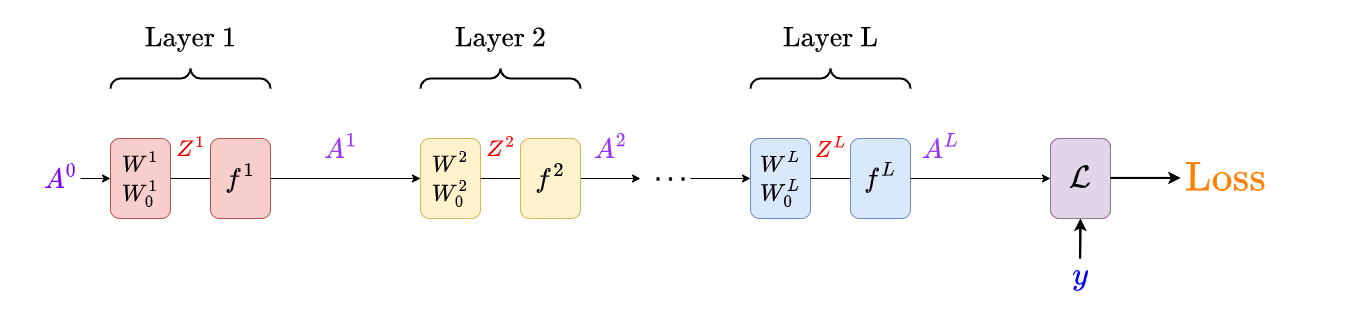
\includegraphics[width=180mm,scale=0.4]{images/nn_1_5_images/network_bp_full.png}
            \caption*{Pretty much the same! Only major difference: swapped scalars for vectors, and vectors for matrices (represented by switching to uppercase)}
        \end{figure}
        
        And, we do backprop the same way, too.
        
        Here, we're not going to explain much as we go: all we're doing is getting the \textbf{derivatives} we need for our \textbf{chain rule}! 
        
        As we go \textbf{backwards}, we can build the gradient for each \textbf{weight} we come across, in the way we described above.
        
        As always, we start from the loss function:
        
        \begin{figure}[H]
            \centering
            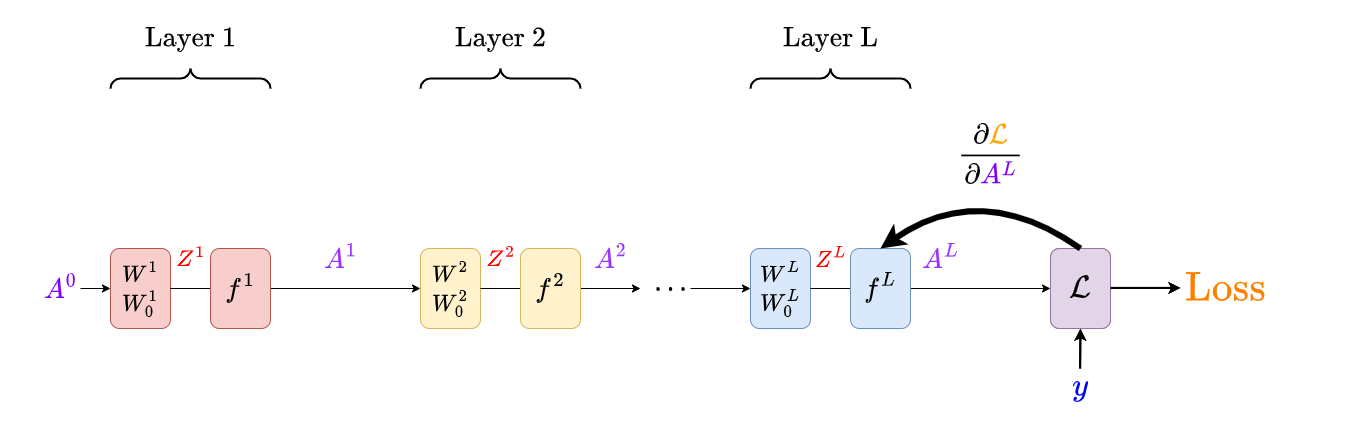
\includegraphics[width=180mm,scale=0.4]{images/nn_1_5_images/network_bp_full1.png}
        \end{figure}
        
        Take another step:
        
        \begin{figure}[H]
            \centering
            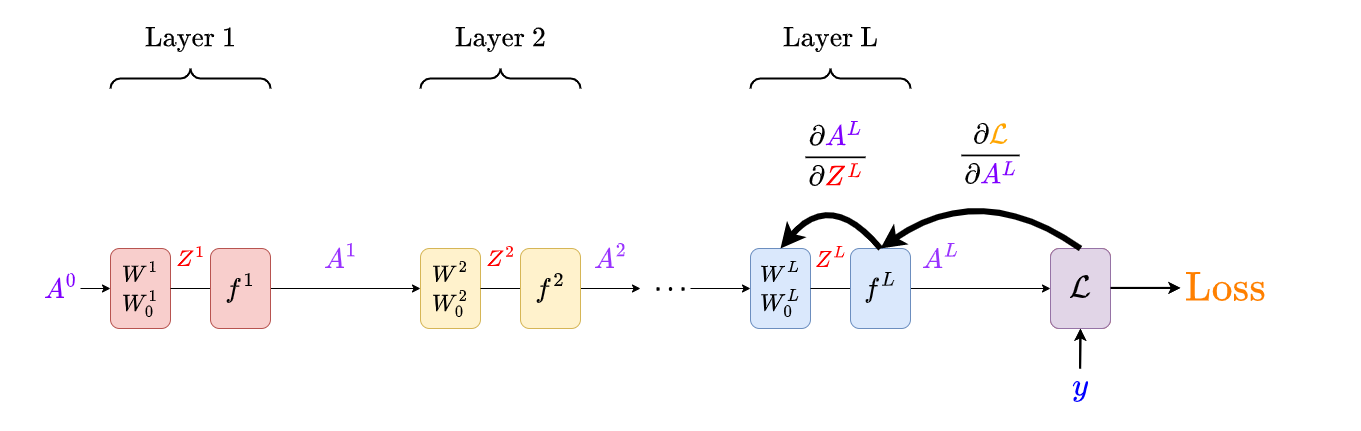
\includegraphics[width=180mm,scale=0.4]{images/nn_1_5_images/network_bp_full2.png}
        \end{figure}
        
        We'll pick up the pace: we'll jump to layer 2 and get its gradient.
            \note{The term $\pderivslash{\red{Z^L}}{\pur{A^2}}$ contains lots of derivatives from every layer between $L$ and 2. \\
            
            But, all we're omitting is the same kinds of steps we're doing in layers 1, 2, and L.}
        
        \begin{figure}[H]
            \centering
            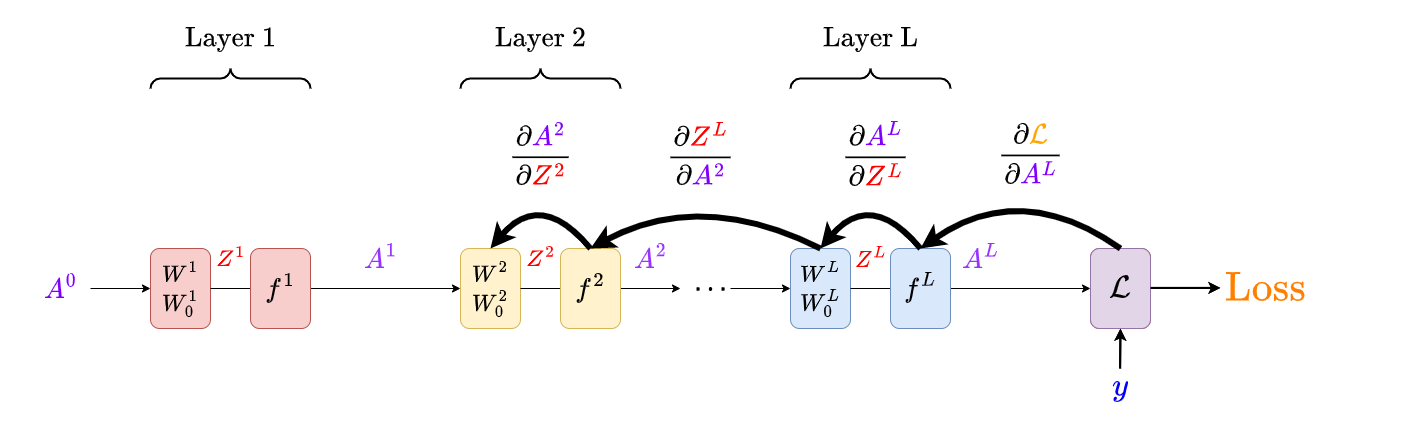
\includegraphics[width=180mm,scale=0.4]{images/nn_1_5_images/network_bp_full3.png}
        \end{figure}
        
        Now, we finally get to layer 1!
        
        \begin{figure}[H]
            \centering
            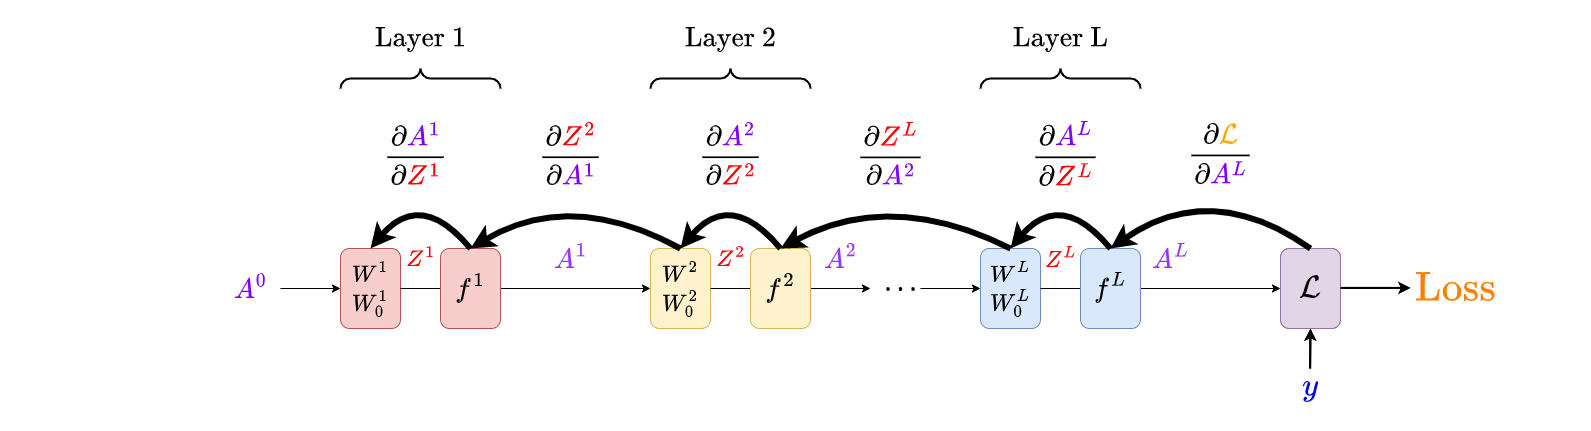
\includegraphics[width=180mm,scale=0.4]{images/nn_1_5_images/network_bp_full4.png}
        \end{figure}
        
        We finish off by getting what we're after: the gradient for $W^1$.\\
        
        \begin{notation}
            We depict neural network gradient descent using the below diagram (outside the box):
            
            The \gren{right}-facing \gren{straight} arrows come \purp{first}: they're part of the \vocab{forward pass}, where we get all of our values.
            
            The \gren{left}-facing \gren{curved} arrows come \purp{after}: they represent the \vocab{back-propagation} of the gradient.
        \end{notation}
        
        \begin{figure}[H]
            \centering
            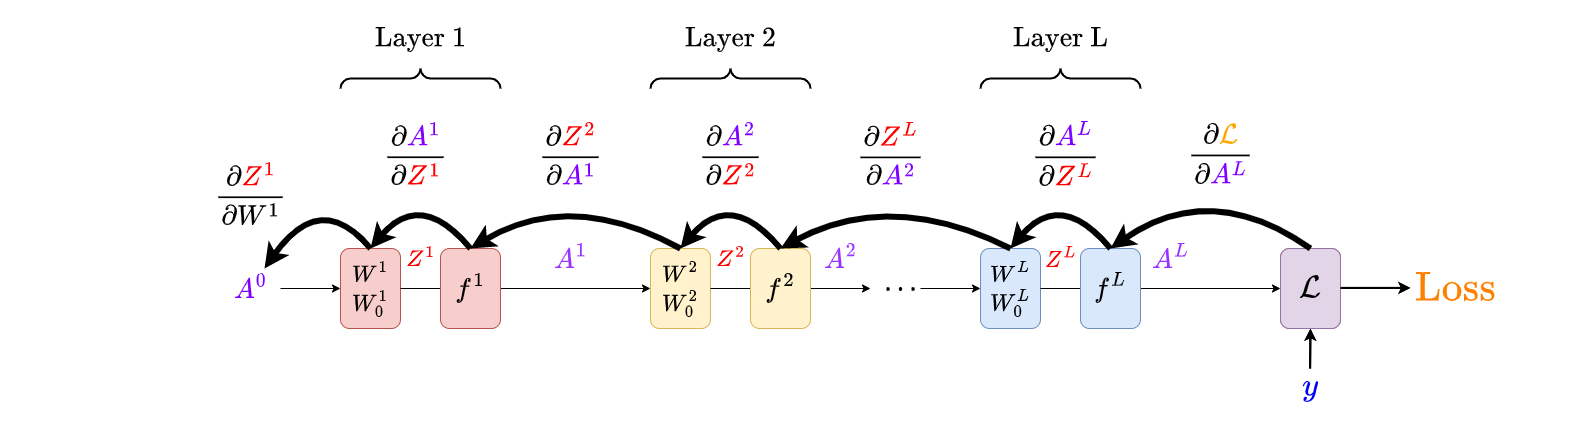
\includegraphics[width=180mm,scale=0.4]{images/nn_1_5_images/network_bp_full5.png}
        \end{figure}
        
        And, with this, we can rewrite our general equation for neural network gradients.
        
    \secdiv
    
    \subsection*{How the Chain Rule changes in Matrix form}
        
        As we discussed before, we can't just add onto our weight gradient to reach another layer: the final term
        
        \begin{equation}
            \pderiv{Z^\ell}{W^\ell}
        \end{equation}
        
        Ends our chain rule when we add it: $W^\ell$ isn't part of the input or output, so it doesn't connect to the previous layer.
        
        So, for this section, we'll add it \textbf{separately} at the end of our chain rule:
        
        \begin{equation*}
            \pderiv {\pur{\loss}} {W^\ell} 
            =
            \overbrace{
                \pderiv {\red{Z^\ell}}   {W^{\ell}}
            }^{\text{Weight link}} 
                \cmul
            \overbrace{
                \Bigg(
                    \pderiv {\pur{\loss}} {\red{Z^\ell}}
                \Bigg)^T
            }^{\text{Other layers}}
        \end{equation*}
        
        That way, we can add onto $\pderivslash {\pur{\loss}} {\red{Z^\ell}}$ without worrying about the weight derivative.
            
        Notice two minor changes caused by the switch to matrices:
        
        \begin{itemize}
            \item The order has to be \textbf{reversed}.
            \item We also have to do some weird \textbf{transposing}.
        \end{itemize}
        
        Both of these mostly boil down to trying to be careful about \textbf{shape}/dimension agreement.
            \note{There are also deeper interpretations, but they aren't worth digging into for now.}\\
        
        \begin{notation}
            The \vocab{gradient} $\nabla_{W^\ell} \loss$ for a neural network is given as:
            
            \begin{equation*}
                \pderiv {\pur{\loss}} {W^\ell} 
                =
                \overbrace{
                    \pderiv {\red{Z^\ell}}   {W^{\ell}}
                }^{\text{Weight link}} 
                    \cmul
                \overbrace{
                    \Bigg(
                        \pderiv {\pur{\loss}} {\red{Z^\ell}}
                    \Bigg)^T
                }^{\text{Other layers}}
            \end{equation*}
            
            We get our remaining terms $\pderivslash {\pur{\loss}} {\red{Z^\ell}}$ by our usual chain rule:
            
            \begin{equation*}
                \pderiv {\pur{\loss}} {Z^\ell}
                =
                \overbrace{
                    \Bigg(
                        \pderiv {\blu{A^\ell}}   {\red{Z^\ell}}
                    \Bigg) 
                }^{\text{Layer $\ell$}}
                \cdot
                \Bigg(
                    \cdots 
                \Bigg)
                \cdot
                \overbrace{
                    \Bigg(
                        \pderiv {\red{Z^{L-1}}}   {A^{L-2}}
                            \cmul
                        \pderiv {\blu{A^{L-1}}}   {\red{Z^{L-1}}}
                    \Bigg) 
                }^{\text{Layer $L-1$}}
                \cdot
                \overbrace{
                    \Bigg(
                        \pderiv {\red{Z^L}}   {A^{L-1}}
                            \cmul
                        \pderiv {\blu{A^L}}   {\red{Z^L}}
                    \Bigg) 
                }^{\text{Layer $L$}}
                \cdot
                \overbrace{
                    \Bigg(
                        \pderiv {\pur{\loss}} {\blu{A^L}} 
                    \Bigg)
                }^{\text{Loss unit}}
            \end{equation*}
        \end{notation}
        
        This is likely our most important equation in this chapter!
        